%%%% Small single column format, used for CIE, CSUR, DTRAP, JACM, JDIQ, JEA, JERIC, JETC, PACMCGIT, TAAS, TACCESS, TACO, TALG, TALLIP (formerly TALIP), TCPS, TDSCI, TEAC, TECS, THRI, TIIS, TIOT, TISSEC, TIST, TKDD, TMIS, TOCE, TOCHI, TOCL, TOCS, TOCT, TODAES, TODS, TOIS, TOIT, TOMACS, TOMM (formerly TOMCCAP), TOMPECS, TOMS, TOPC, TOPLAS, TOPS, TOS, TOSEM, TOSN, TRETS, TSAS, TSC, TSLP, TWEB.
% \documentclass[format=acmsmall, review=false, screen=true]{acmart}

%%%% Large single column format, used for IMWUT, JOCCH, PACMPL, POMACS, TAP, PACMHCI
\documentclass[acmlarge]{acmart}
%%%% Large double column format, used for TOG
% \documentclass[acmtog, authorversion]{acmart}

%%%% Generic manuscript mode
%\documentclass[manuscript, review, screen]{acmart}
%\setcitestyle{super,sort&compress}
%\citestyle{acmnumeric}
\usepackage{booktabs} % For formal tables
%\usepackage{hyperref}

%\usepackage[ruled]{algorithm2e} % For algorithms
%\usepackage{listings}
%\usepackage{glossaries} % For abbreviations
%\usepackage[acronym,nonumberlist]{glossaries-extra}

%\loadglsentries{acronym_list}


% Load basic packages
%\usepackage{balance}       % to better equalize the last page
%\usepackage{graphics}      % for EPS, load graphicx instead
%\usepackage[T1]{fontenc}   % for umlauts and other diaeresis
%\usepackage{txfonts}
%\usepackage{mathptmx}
%\usepackage[pdflang={en-US},pdftex]{hyperref}
%%\usepackage{color}
%%\usepackage{booktabs}
%%\usepackage{textcomp}
%%\usepackage{gensymb}



% Package for algorithmic code
\usepackage{algorithm}
\usepackage[noend]{algpseudocode}
\usepackage{subcaption}
\makeatletter
\def\BState{\State\hskip-\ALG@thistlm}
\makeatother


% Metadata Information
%\acmJournal{IMWUT}
%\acmVolume{0}
%\acmNumber{0}
%\acmArticle{0}
%\acmYear{2018}
%\acmMonth{3}

%\acmBadgeL[http://ctuning.org/ae/ppopp2016.html]{ae-logo}
%\acmBadgeR[http://ctuning.org/ae/ppopp2016.html]{ae-logo}

% Copyright
%\setcopyright{acmcopyright}
%\setcopyright{acmlicensed}
%\setcopyright{rightsretained}
%\setcopyright{usgov}
\setcopyright{usgovmixed}
%\setcopyright{cagov}
%\setcopyright{cagovmixed}

% DOI
%\acmDOI{0000001.0000001}


% Document starts
\begin{document}


% Title portion
\title{Fancy title}

\author{Xi}
%\orcid{1234-5678-9012-3456}
\affiliation{%
  \institution{Distributed \& Interactive Systems, Centrum Wiskunde \& Informatica}
  \city{Science Park 123, 1098 XG, Amsterdam}
  \country{The Netherlands}}
\email{X@cwi.nl}

%\author{Shashank Rao}
%%\orcid{1234-5678-9012-3456}
%\affiliation{%
%  \institution{Multimedia Computing, TU Delft}
%  \city{Mekelweg 4, 2628 CD Delft}
%  \country{The Netherlands}}
%\email{s.p.rao@student.tudelft.nl}

\author{XYZ}
%\orcid{1234-5678-9012-3456}
\affiliation{%
  \institution{Distributed \& Interactive Systems, Centrum Wiskunde \& Informatica}
  \city{Science Park 123, 1098 XG, Amsterdam}
  \country{The Netherlands}}
\email{p.s.cesar@cwi.nl}



\renewcommand\shortauthors{X. et al.}

%\begin{abstract}
%
%
%\end{abstract}

\keywords{fancy keywords}

\maketitle

\section*{Abstract}
\textbf{Purpose:}  \\

\noindent \textbf{Methods:}  
\\

%
%\begin{figure}[t]
%\centering
%\begin{subfigure}{0.30\textwidth}
%%\hskip-1cm
%\centering
%  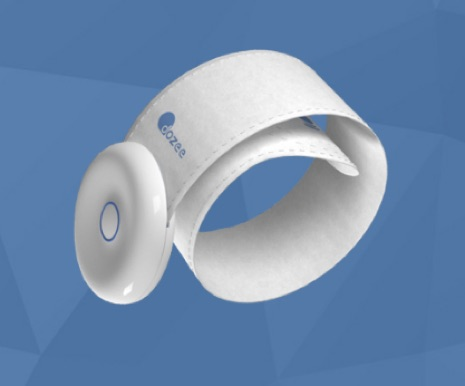
\includegraphics[scale=0.11]{images/dozee_device.jpg}
%  \caption{Dozee sleep-monitoring device.}
%  \label{fig:doz}
%\end{subfigure}
%% \hfill
%\begin{subfigure}{0.30\textwidth}
%\centering
%  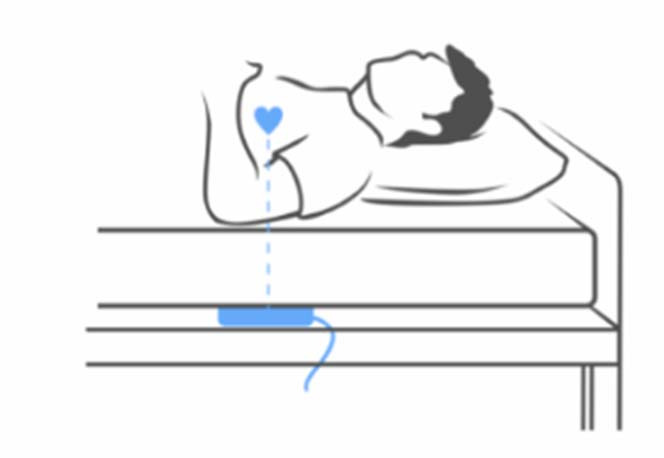
\includegraphics[scale=0.11]{images/dozee.jpeg}
%  \caption{Placement of Dozee sensor-sheet}
%  \label{fig:dozee_use}
%\end{subfigure}
%
%	\caption{\textbf{Dozee sensor-sheet and its usage}}
%	\label{fig:dozee}
%\end{figure}
%


\noindent \textbf{Results:} 



\bibliographystyle{ACM-Reference-Format}
\bibliography{report}
\end{document}
